A Figura~\ref{fig:comparacao_decrescente} apresenta a comparação entre
os sete algoritmos para entradas inicialmente organizadas em ordem
decrescente.

\begin{figure}[H]
    \centering
    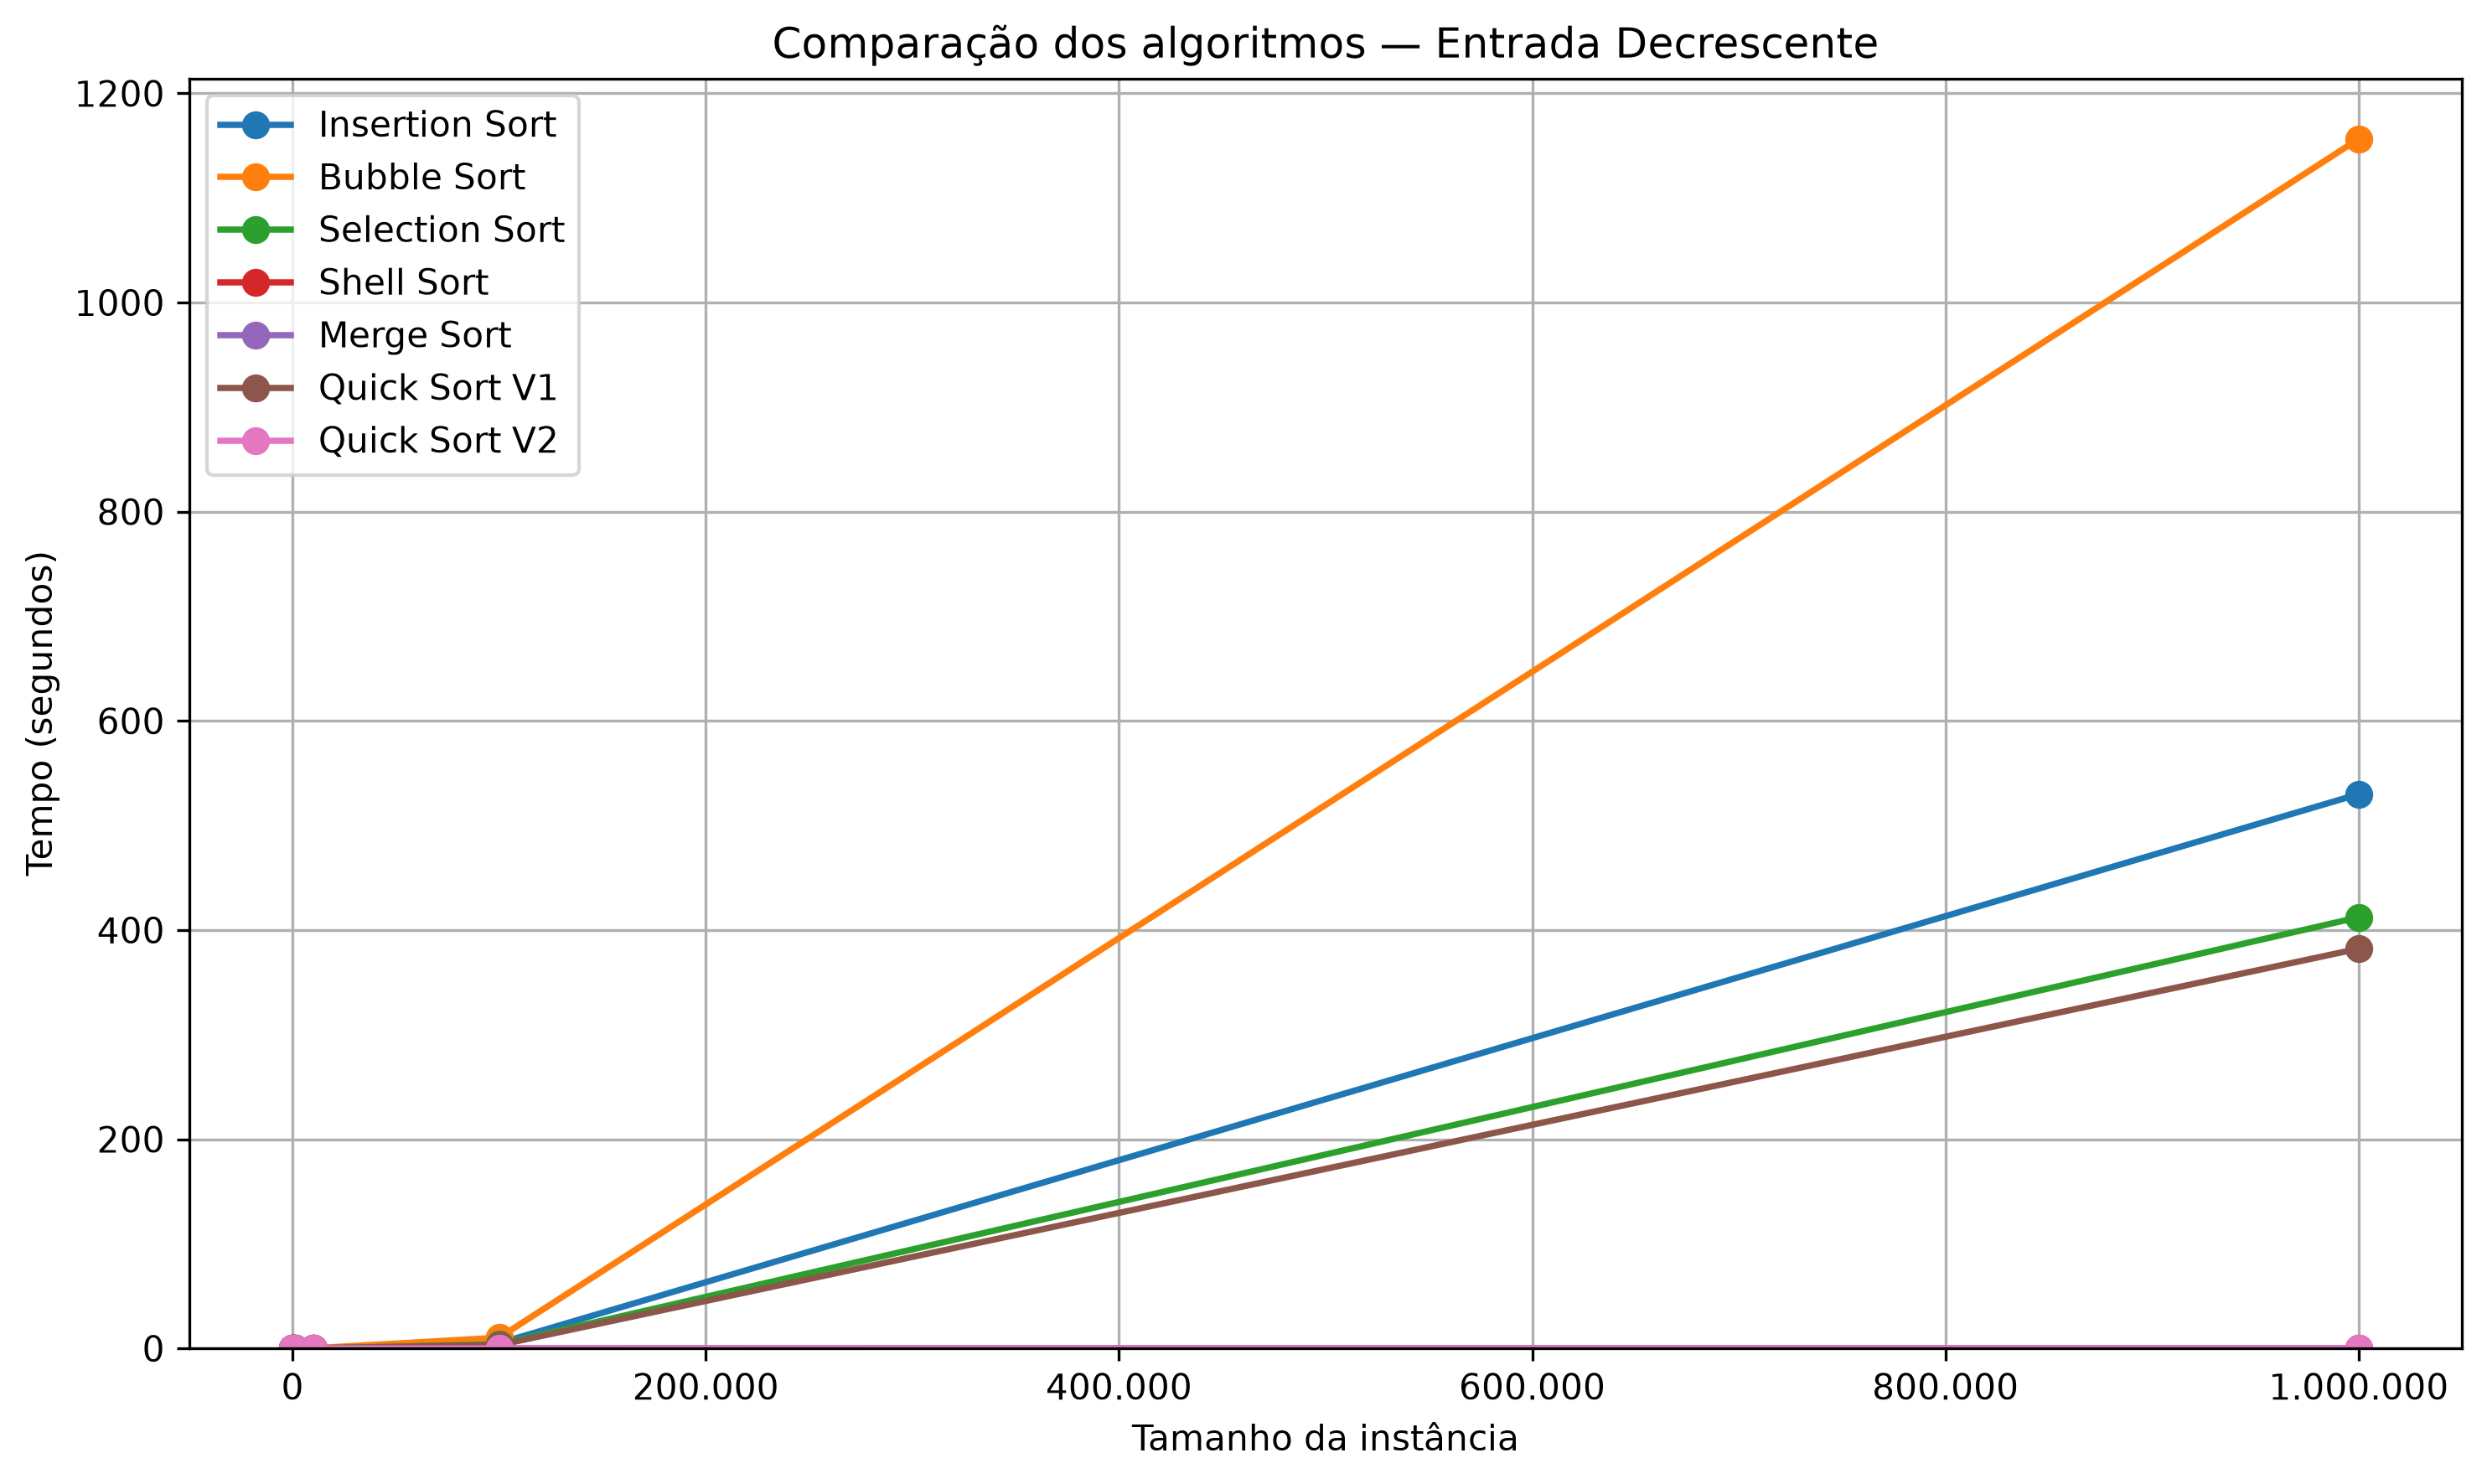
\includegraphics[width=\textwidth,keepaspectratio]{Imagens/Comparacoes/comparacao_decrescente.png}
    \caption{Comparação dos algoritmos para entrada decrescente.}
    \label{fig:comparacao_decrescente}
\end{figure}

Nesse caso, quatro algoritmos apresentaram tempos elevados para
1.000.000 de elementos. O \textit{Bubble Sort} foi o mais lento, com
cerca de 1150 segundos, devido à grande quantidade de comparações e
trocas necessárias para inverter completamente o vetor. Em seguida
aparece o \textit{Insertion Sort}, com cerca de 530 segundos, pois cada
novo elemento precisa ser deslocado até o início da parte já ordenada.
Esse valor é aproximadamente o dobro do observado em entradas
aleatórias, o que é coerente com o fato de o número de deslocamentos
no pior caso ser cerca de duas vezes o do caso médio.

O \textit{Selection Sort}, com cerca de 410 segundos, apresentou tempo
muito próximo ao observado nas entradas crescente e aleatória, pois o
número de comparações realizadas não depende da organização inicial do
vetor. O \textit{Quick Sort} versão 1 apresentou cerca de 380 segundos:
em um vetor decrescente, o primeiro elemento é o maior valor da
partição, e o particionamento separa apenas um elemento por vez, o que
leva o algoritmo ao pior caso quadrático.

O \textit{Shell Sort}, o \textit{Merge Sort} e o \textit{Quick Sort}
versão 2 apresentaram tempos muito baixos, praticamente indistinguíveis
do eixo horizontal na escala do gráfico. No caso do \textit{Merge Sort},
isso ocorre porque as etapas de divisão e intercalação são as mesmas
independentemente da disposição inicial dos elementos. Na versão 2 do
\textit{Quick Sort}, a média aritmética manteve as partições
equilibradas, evitando o pior caso observado na versão 1.